\chapter{Optimising code}\label{profiling}

\begin{quote}
``Programmers waste enormous amounts of time thinking about, or worrying
about, the speed of noncritical parts of their programs, and these
attempts at efficiency actually have a strong negative impact when
debugging and maintenance are considered.''

--- Donald Knuth.
\end{quote}

Optimising code to make it run faster is an iterative process:
\index{optimisation}

\begin{enumerate}
\def\labelenumi{\arabic{enumi}.}
\itemsep1pt\parskip0pt\parsep0pt
\item
  Find the biggest bottleneck (the slowest part of your code).
\item
  Try to eliminate it (you may not succeed but that's ok).
\item
  Repeat until your code is ``fast enough.''
\end{enumerate}

This sounds easy, but it's not.

Even experienced programmers have a hard time identifying bottlenecks in
their code. Instead of relying on your intuition, you should
\textbf{profile} your code: use realistic inputs and measure the
run-time of each individual operation. Only once you've identified the
most important bottlenecks can you attempt to eliminate them. It's
difficult to provide general advice on improving performance, but I try
my best with six techniques that can be applied in many situations. I'll
also suggest a general strategy for performance optimisation that helps
ensure that your faster code will still be correct code.

It's easy to get caught up in trying to remove all bottlenecks. Don't!
Your time is valuable and is better spent analysing your data, not
eliminating possible inefficiencies in your code. Be pragmatic: don't
spend hours of your time to save seconds of computer time. To enforce
this advice, you should set a goal time for your code and optimise only
up to that goal. This means you will not eliminate all bottlenecks. Some
you will not get to because you've met your goal. Others you may need to
pass over and accept either because there is no quick and easy solution
or because the code is already well optimised and no significant
improvement is possible. Accept these possibilities and move on to the
next candidate. \index{bottlenecks}

\paragraph{Outline}

\begin{itemize}
\item
  \hyperref[measure-perf]{Measuring performance} describes how to find
  the bottlenecks in your code using line profiling.
\item
  \hyperref[improve-perf]{Improving performance} outlines seven general
  strategies for improving the performance of your code.
\item
  \hyperref[code-organisation]{Code organisation} teaches you how to
  organise your code to make optimisation as easy, and bug free, as
  possible.
\item
  \hyperref[already-solved]{Already solved} reminds you to look for
  existing solutions.
\item
  \hyperref[be-lazy]{Do as little as possible} emphasises the importance
  of being lazy: often the easiest way to make a function faster is to
  let it to do less work.
\item
  \hyperref[vectorise]{Vectorise} concisely defines vectorisation, and
  shows you how to make the most of built-in functions.
\item
  \hyperref[avoid-copies]{Avoid copies} discusses the performance perils
  of copying data.
\item
  \hyperref[byte-code]{Byte code compilation} shows you how to take
  advantage of R's byte code compiler.
\item
  \hyperref[t-test]{Case study: t-test} pulls all the pieces together
  into a case study showing how to speed up repeated t-tests by
  \textasciitilde{}1000x.
\item
  \hyperref[parallelise]{Parallelise} teaches you how to use
  parallelisation to spread computation across all the cores in your
  computer.
\item
  \hyperref[more-techniques]{Other techniques} finishes the chapter with
  pointers to more resources that will help you write fast code.
\end{itemize}

\paragraph{Prerequisites}

In this chapter we'll be using the \texttt{lineprof} package to
understand the performance of R code. Get it with:

\begin{Shaded}
\begin{Highlighting}[]
\NormalTok{devtools::}\KeywordTok{install_github}\NormalTok{(}\StringTok{"hadley/lineprof"}\NormalTok{)}
\end{Highlighting}
\end{Shaded}

\hyperdef{}{measure-perf}{\section{Measuring
performance}\label{measure-perf}}

To understand performance, you use a profiler. There are a number of
different types of profilers. R uses a fairly simple type called a
sampling or statistical profiler. A sampling profiler stops the
execution of code every few milliseconds and records which function is
currently executing (along with which function called that function, and
so on). For example, consider \texttt{f()}, below: \index{profiling}
\index{performance!measuring}

\begin{Shaded}
\begin{Highlighting}[]
\KeywordTok{library}\NormalTok{(lineprof)}
\NormalTok{f <-}\StringTok{ }\NormalTok{function() \{}
  \KeywordTok{pause}\NormalTok{(}\FloatTok{0.1}\NormalTok{)}
  \KeywordTok{g}\NormalTok{()}
  \KeywordTok{h}\NormalTok{()}
\NormalTok{\}}
\NormalTok{g <-}\StringTok{ }\NormalTok{function() \{}
  \KeywordTok{pause}\NormalTok{(}\FloatTok{0.1}\NormalTok{)}
  \KeywordTok{h}\NormalTok{()}
\NormalTok{\}}
\NormalTok{h <-}\StringTok{ }\NormalTok{function() \{}
  \KeywordTok{pause}\NormalTok{(}\FloatTok{0.1}\NormalTok{)}
\NormalTok{\}}
\end{Highlighting}
\end{Shaded}

(I use \texttt{pause()} instead of \texttt{Sys.sleep()} because
\texttt{Sys.sleep()} does not appear in profiling outputs because as far
as R can tell, it doesn't use up any computing time.) \indexc{pause()}

If we profiled the execution of \texttt{f()}, stopping the execution of
code every 0.1 s, we'd see a profile like below. Each line represents
one ``tick'' of the profiler (0.1 s in this case), and function calls
are nested with \texttt{\textgreater{}}. It shows that the code spends
0.1 s running \texttt{f()}, then 0.2 s running \texttt{g()}, then 0.1 s
running \texttt{h()}.

\begin{verbatim}
f() 
f() > g()
f() > g() > h()
f() > h()
\end{verbatim}

If we actually profile \texttt{f()}, using the code below, we're
unlikely to get such a clear result.

\begin{Shaded}
\begin{Highlighting}[]
\NormalTok{tmp <-}\StringTok{ }\KeywordTok{tempfile}\NormalTok{()}
\KeywordTok{Rprof}\NormalTok{(tmp, }\DataTypeTok{interval =} \FloatTok{0.1}\NormalTok{)}
\KeywordTok{f}\NormalTok{()}
\KeywordTok{Rprof}\NormalTok{(}\OtherTok{NULL}\NormalTok{)}
\end{Highlighting}
\end{Shaded}

That's because profiling is hard to do accurately without slowing your
code down by many orders of magnitude. The compromise that
\texttt{RProf()} makes, sampling, only has minimal impact on the overall
performance, but is fundamentally stochastic. There's some variability
in both the accuracy of the timer and in the time taken by each
operation, so each time you profile you'll get a slightly different
answer. Fortunately, pinpoint accuracy is not needed to identify the
slowest parts of your code. \indexc{RProf()}

Rather than focussing on individual calls, we'll visualise aggregates
using the lineprof package. There are a number of other options, like
\texttt{summaryRprof()}, the proftools package, and the profr package,
but these tools are beyond the scope of this book. I wrote the
\texttt{lineprof} package as a simpler way to visualise profiling data.
As the name suggests, the fundamental unit of analysis in
\texttt{lineprof()} is a line of code. This makes lineprof less precise
than the alternatives (because a line of code can contain multiple
function calls), but it's easier to understand the context.

To use \texttt{lineprof}, we first save the code in a file and
\texttt{source()} it. Here \texttt{profiling-example.R} contains the
definition of \texttt{f()}, \texttt{g()}, and \texttt{h()}. Note that
you \emph{must} use \texttt{source()} to load the code. This is because
lineprof uses srcrefs to match up the code to the profile, and the
needed srcrefs are only created when you load code from disk. We then
use \texttt{lineprof()} to run our function and capture the timing
output. Printing this object shows some basic information. For now,
we'll just focus on the time column which estimates how long each line
took to run and the ref column which tells us which line of code was
run. The estimates aren't perfect, but the ratios look about right.
\index{line profiling}

\begin{Shaded}
\begin{Highlighting}[]
\KeywordTok{library}\NormalTok{(lineprof)}
\KeywordTok{source}\NormalTok{(}\StringTok{"profiling-example.R"}\NormalTok{)}
\NormalTok{l <-}\StringTok{ }\KeywordTok{lineprof}\NormalTok{(}\KeywordTok{f}\NormalTok{())}
\NormalTok{l}
\CommentTok{#>    time alloc release dups           ref     src}
\CommentTok{#> 1 0.074 0.001       0    0 profiling.R#2 f/pause}
\CommentTok{#> 2 0.143 0.002       0    0 profiling.R#3 f/g    }
\CommentTok{#> 3 0.071 0.000       0    0 profiling.R#4 f/h   }
\end{Highlighting}
\end{Shaded}

lineprof provides some functions to navigate through this data
structure, but they're a bit clumsy. Instead, we'll start an interactive
explorer using the shiny package. \texttt{shine(l)} will open a new web
page (or if you're using RStudio, a new pane) that shows your source
code annotated with information about how long each line took to run.
\texttt{shine()} starts a shiny app which ``blocks'' your R session. To
exit, you'll need to stop the process using escape or ctrl + c.

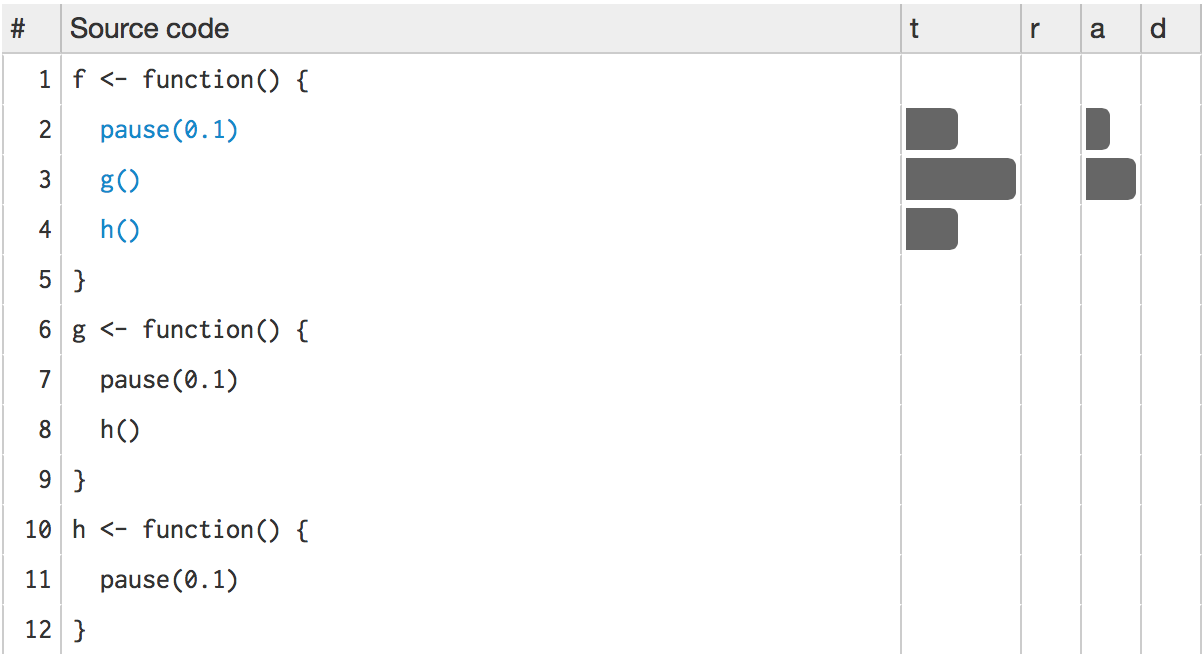
\includegraphics[width=4.35in]{screenshots/profiling-lineprof-f.png}

The \texttt{t} column visualises how much time is spent on each line.
(You'll learn about the other columns in
\hyperref[memory-profiling]{memory profiling}.) While not precise, it
allows you to spot bottlenecks, and you can get precise numbers by
hovering over each bar. This shows that twice as much time is spent on
\texttt{g()} as on \texttt{h()}, so it would make sense to drill down
into \texttt{g()} for more details. To do so, click \texttt{g()}:

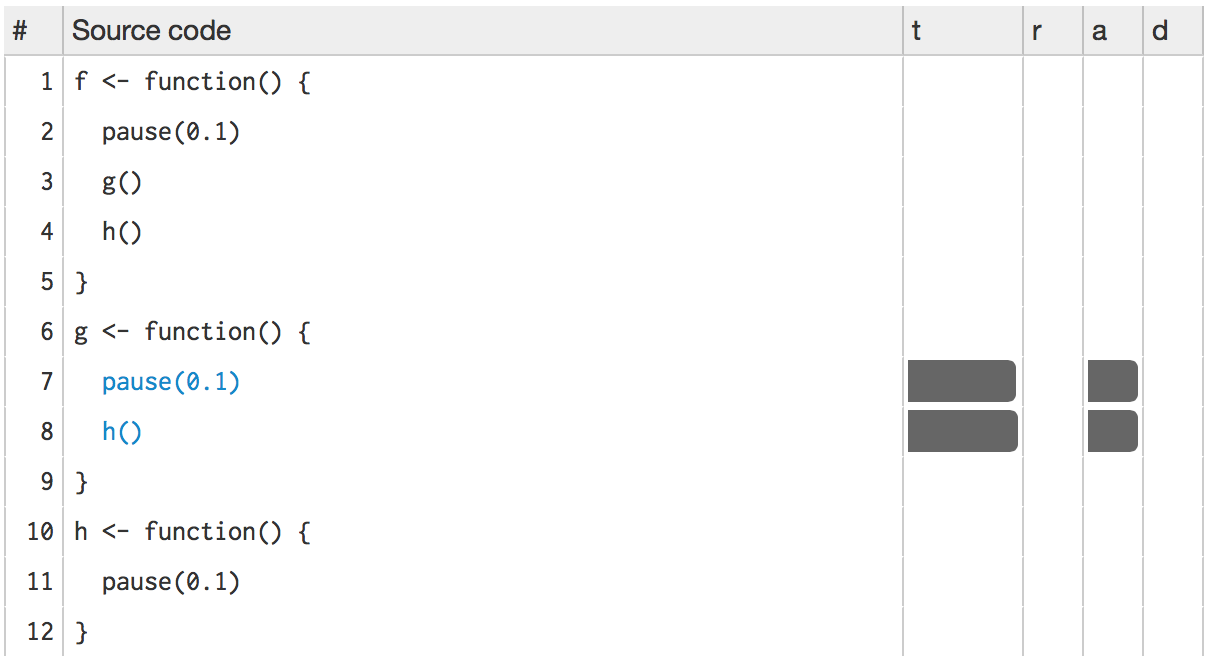
\includegraphics[width=4.35in]{screenshots/profiling-lineprof-g.png}

Then \texttt{h()}:

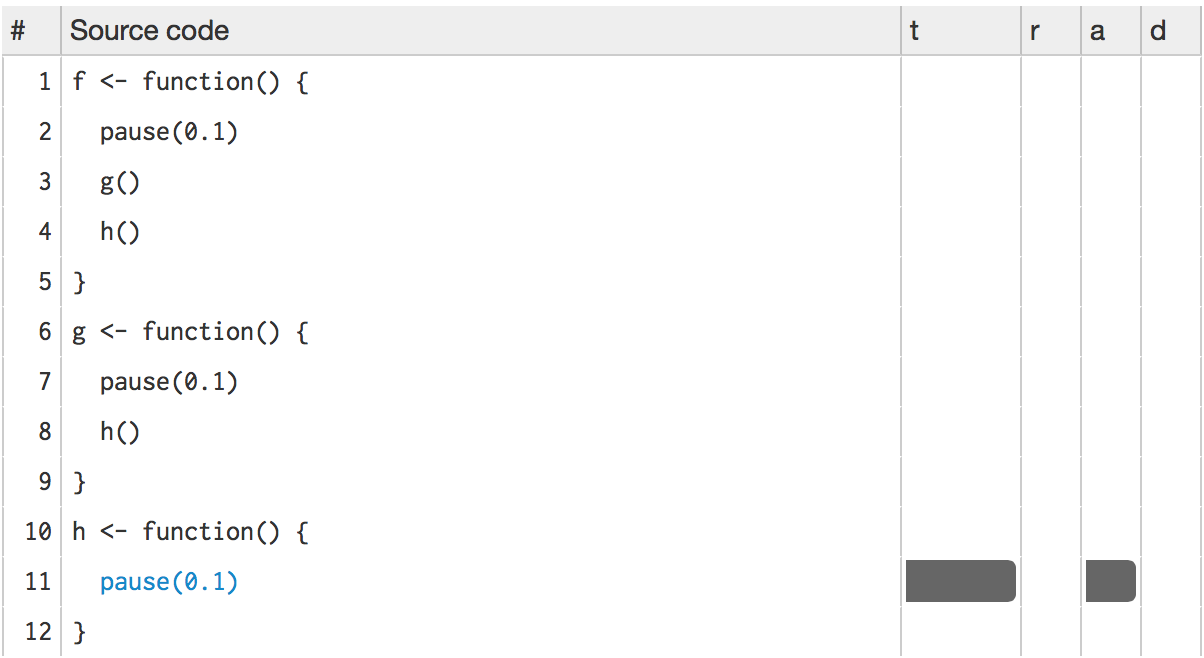
\includegraphics[width=4.35in]{screenshots/profiling-lineprof-h.png}

This technique should allow you to quickly identify the major
bottlenecks in your code.

\subsection{Limitations}

There are some other limitations to profiling:

\begin{itemize}
\item
  Profiling does not extend to C code. You can see if your R code calls
  C/C++ code but not what functions are called inside of your C/C++
  code. Unfortunately, tools for profiling compiled code are beyond the
  scope of this book (i.e., I have no idea how to do it).
\item
  Similarly, you can't see what's going on inside primitive functions or
  byte code compiled code.
\item
  If you're doing a lot of functional programming with anonymous
  functions, it can be hard to figure out exactly which function is
  being called. The easiest way to work around this is to name your
  functions.
\item
  Lazy evaluation means that arguments are often evaluated inside
  another function. For example, in the following code, profiling would
  make it seem like \texttt{i()} was called by \texttt{j()} because the
  argument isn't evaluated until it's needed by \texttt{j()}.

\begin{Shaded}
\begin{Highlighting}[]
\NormalTok{i <-}\StringTok{ }\NormalTok{function() \{}
  \KeywordTok{pause}\NormalTok{(}\FloatTok{0.1}\NormalTok{)}
  \DecValTok{10}
\NormalTok{\}}
\NormalTok{j <-}\StringTok{ }\NormalTok{function(x) \{}
  \NormalTok{x +}\StringTok{ }\DecValTok{10}
\NormalTok{\}}
\KeywordTok{j}\NormalTok{(}\KeywordTok{i}\NormalTok{())}
\end{Highlighting}
\end{Shaded}

  If this is confusing, you can create temporary variables to force
  computation to happen earlier.
\end{itemize}

\hyperdef{}{improve-perf}{\section{Improving
performance}\label{improve-perf}}

\begin{quote}
``We should forget about small efficiencies, say about 97\% of the time:
premature optimization is the root of all evil. Yet we should not pass
up our opportunities in that critical 3\%. A good programmer will not be
lulled into complacency by such reasoning, he will be wise to look
carefully at the critical code; but only after that code has been
identified.''

--- Donald Knuth.
\end{quote}

Once you've used profiling to identify a bottleneck, you need to make it
faster. The following sections introduce you to a number of techniques
that I've found broadly useful: \index{improving performance}
\index{performance!improving}

\begin{enumerate}
\def\labelenumi{\arabic{enumi}.}
\itemsep1pt\parskip0pt\parsep0pt
\item
  Look for existing solutions.
\item
  Do less work.
\item
  Vectorise.
\item
  Parallelise.
\item
  Avoid copies.
\item
  Byte-code compile.
\end{enumerate}

A final technique is to rewrite in a faster language, like C++. That's a
big topic and is covered in \hyperref[rcpp]{Rcpp}.

Before we get into specific techniques, I'll first describe a general
strategy and organisational style that's useful when working on
performance.

\hyperdef{}{code-organisation}{\section{Code
organisation}\label{code-organisation}}

There are two traps that are easy to fall into when trying to make your
code faster:

\begin{enumerate}
\def\labelenumi{\arabic{enumi}.}
\itemsep1pt\parskip0pt\parsep0pt
\item
  Writing faster but incorrect code.
\item
  Writing code that you think is faster, but is actually no better.
\end{enumerate}

The strategy outlined below will help you avoid these pitfalls.
\index{improving performance!strategy}

When tackling a bottleneck, you're likely to come up with multiple
approaches. Write a function for each approach, encapsulating all
relevant behaviour. This makes it easier to check that each approach
returns the correct result and to time how long it takes to run. To
demonstrate the strategy, I'll compare two approaches for computing the
mean:

\begin{Shaded}
\begin{Highlighting}[]
\NormalTok{mean1 <-}\StringTok{ }\NormalTok{function(x) }\KeywordTok{mean}\NormalTok{(x)}
\NormalTok{mean2 <-}\StringTok{ }\NormalTok{function(x) }\KeywordTok{sum}\NormalTok{(x) /}\StringTok{ }\KeywordTok{length}\NormalTok{(x)}
\end{Highlighting}
\end{Shaded}

I recommend that you keep a record of everything you try, even the
failures. If a similar problem occurs in the future, it'll be useful to
see everything you've tried. To do this I often use R Markdown, which
makes it easy to intermingle code with detailed comments and notes.

Next, generate a representative test case. The case should be big enough
to capture the essence of your problem but small enough that it takes
only a few seconds to run. You don't want it to take too long because
you'll need to run the test case many times to compare approaches. On
the other hand, you don't want the case to be too small because then
results might not scale up to the real problem.

Use this test case to quickly check that all variants return the same
result. An easy way to do so is with \texttt{stopifnot()} and
\texttt{all.equal()}. For real problems with fewer possible outputs, you
may need more tests to make sure that an approach doesn't accidentally
return the correct answer. That's unlikely for the mean.
\indexc{stopifnot()}

\begin{Shaded}
\begin{Highlighting}[]
\NormalTok{x <-}\StringTok{ }\KeywordTok{runif}\NormalTok{(}\DecValTok{100}\NormalTok{)}
\KeywordTok{stopifnot}\NormalTok{(}\KeywordTok{all.equal}\NormalTok{(}\KeywordTok{mean1}\NormalTok{(x), }\KeywordTok{mean2}\NormalTok{(x)))}
\end{Highlighting}
\end{Shaded}

Finally, use the \texttt{microbenchmark} package to compare how long
each variation takes to run. For bigger problems, reduce the
\texttt{times} parameter so that it only takes a couple of seconds to
run. Focus on the median time, and use the upper and lower quartiles to
gauge the variability of the measurement. \indexc{microbenchmark()}

\begin{Shaded}
\begin{Highlighting}[]
\KeywordTok{microbenchmark}\NormalTok{(}
  \KeywordTok{mean1}\NormalTok{(x),}
  \KeywordTok{mean2}\NormalTok{(x)}
\NormalTok{)}
\CommentTok{#> Unit: nanoseconds}
\CommentTok{#>      expr   min    lq median    uq    max neval}
\CommentTok{#>  mean1(x) 5,030 5,260  5,400 5,660 47,100   100}
\CommentTok{#>  mean2(x)   709   808  1,020 1,140 35,900   100}
\end{Highlighting}
\end{Shaded}

(You might be surprised by the results: \texttt{mean(x)} is considerably
slower than \texttt{sum(x) / length(x)}. This is because, among other
reasons, \texttt{mean(x)} makes two passes over the vector to be more
numerically accurate.)

Before you start experimenting, you should have a target speed that
defines when the bottleneck is no longer a problem. Setting such a goal
is important because you don't want to spend valuable time
over-optimising your code.

If you'd like to see this strategy in action, I've used it a few times
on stackoverflow:

\begin{itemize}
\itemsep1pt\parskip0pt\parsep0pt
\item
  \url{http://stackoverflow.com/questions/22515525\#22518603}
\item
  \url{http://stackoverflow.com/questions/22515175\#22515856}
\item
  \url{http://stackoverflow.com/questions/3476015\#22511936}
\end{itemize}

\hyperdef{}{already-solved}{\section{Has someone already solved the
problem?}\label{already-solved}}

Once you've organised your code and captured all the variations you can
think of, it's natural to see what others have done. You are part of a
large community, and it's quite possible that someone has already
tackled the same problem. If your bottleneck is a function in a package,
it's worth looking at other packages that do the same thing. Two good
places to start are:

\begin{itemize}
\item
  \href{http://cran.rstudio.com/web/views/}{CRAN task views}. If there's
  a CRAN task view related to your problem domain, it's worth looking at
  the packages listed there.
\item
  Reverse dependencies of Rcpp, as listed on its
  \href{http://cran.r-project.org/web/packages/Rcpp}{CRAN page}. Since
  these packages use C++, it's possible to find a solution to your
  bottleneck written in a higher performance language.
\end{itemize}

Otherwise, the challenge is describing your bottleneck in a way that
helps you find related problems and solutions. Knowing the name of the
problem or its synonyms will make this search much easier. But because
you don't know what it's called, it's hard to search for it! By reading
broadly about statistics and algorithms, you can build up your own
knowledge base over time. Alternatively, ask others. Talk to your
colleagues and brainstorm some possible names, then search on Google and
stackoverflow. It's often helpful to restrict your search to R related
pages. For Google, try \href{http://www.rseek.org/}{rseek}. For
stackoverflow, restrict your search by including the R tag,
\texttt{{[}R{]}}, in your search. \index{searching}

As discussed above, record all solutions that you find, not just those
that immediately appear to be faster. Some solutions might be initially
slower, but because they are easier to optimise they end up being
faster. You may also be able to combine the fastest parts from different
approaches. If you've found a solution that's fast enough,
congratulations! If appropriate, you may want to share your solution
with the R community. Otherwise, read on.

\subsection{Exercises}

\begin{enumerate}
\def\labelenumi{\arabic{enumi}.}
\item
  What are faster alternatives to \texttt{lm}? Which are specifically
  designed to work with larger datasets?
\item
  What package implements a version of \texttt{match()} that's faster
  for repeated lookups? How much faster is it?
\item
  List four functions (not just those in base R) that convert a string
  into a date time object. What are their strengths and weaknesses?
\item
  How many different ways can you compute a 1d density estimate in R?
\item
  Which packages provide the ability to compute a rolling mean?
\item
  What are the alternatives to \texttt{optim()}?
\end{enumerate}

\hyperdef{}{be-lazy}{\section{Do as little as possible}\label{be-lazy}}

The easiest way to make a function faster is to let it do less work. One
way to do that is use a function tailored to a more specific type of
input or ouput, or a more specific problem. For example:

\begin{itemize}
\item
  \texttt{rowSums()}, \texttt{colSums()}, \texttt{rowMeans()}, and
  \texttt{colMeans()} are faster than equivalent invocations that use
  \texttt{apply()} because they are vectorised (the topic of the next
  section).
\item
  \texttt{vapply()} is faster than \texttt{sapply()} because it
  pre-specifies the output type.
\item
  If you want to see if a vector contains a single value,
  \texttt{any(x == 10)} is much faster than \texttt{10 \%in\% x}. This
  is because testing equality is simpler than testing inclusion in a
  set.
\end{itemize}

Having this knowledge at your fingertips requires knowing that
alternative functions exist: you need to have a good vocabulary. Start
with \hyperref[vocabulary]{the basics}, and expand your vocab by
regularly reading R code. Good places to read code are the
\href{https://stat.ethz.ch/mailman/listinfo/r-help}{R-help mailing list}
and \href{http://stackoverflow.com/questions/tagged/r}{stackoverflow}.

Some functions coerce their inputs into a specific type. If your input
is not the right type, the function has to do extra work. Instead, look
for a function that works with your data as it is, or consider changing
the way you store your data. The most common example of this problem is
using \texttt{apply()} on a data frame. \texttt{apply()} always turns
its input into a matrix. Not only is this error prone (because a data
frame is more general than a matrix), it is also slower.

Other functions will do less work if you give them more information
about the problem. It's always worthwhile to carefully read the
documentation and experiment with different arguments. Some examples
that I've discovered in the past include:

\begin{itemize}
\item
  \texttt{read.csv()}: specify known column types with
  \texttt{colClasses}.
\item
  \texttt{factor()}: specify known levels with \texttt{levels}.
\item
  \texttt{cut()}: don't generate labels with \texttt{labels = FALSE} if
  you don't need them, or, even better, use \texttt{findInterval()} as
  mentioned in the ``see also'' section of the documentation.
\item
  \texttt{unlist(x, use.names = FALSE)} is much faster than
  \texttt{unlist(x)}.
\item
  \texttt{interaction()}: if you only need combinations that exist in
  the data, use \texttt{drop = TRUE}.
\end{itemize}

Sometimes you can make a function faster by avoiding method dispatch. As
we saw in (\hyperref[extreme-dynamism]{Extreme dynamism}), method
dispatch in R can be costly. If you're calling a method in a tight loop,
you can avoid some of the costs by doing the method lookup only once:
\index{methods!cost of dispatch, avoiding}

\begin{itemize}
\item
  For S3, you can do this by calling \texttt{generic.class()} instead of
  \texttt{generic()}.
\item
  For S4, you can do this by using \texttt{findMethod()} to find the
  method, saving it to a variable, and then calling that function.
\end{itemize}

For example, calling \texttt{mean.default()} quite a bit faster than
calling \texttt{mean()} for small vectors:

\begin{Shaded}
\begin{Highlighting}[]
\NormalTok{x <-}\StringTok{ }\KeywordTok{runif}\NormalTok{(}\FloatTok{1e2}\NormalTok{)}

\KeywordTok{microbenchmark}\NormalTok{(}
  \KeywordTok{mean}\NormalTok{(x),}
  \KeywordTok{mean.default}\NormalTok{(x)}
\NormalTok{)}
\CommentTok{#> Unit: microseconds}
\CommentTok{#>             expr  min   lq median   uq   max neval}
\CommentTok{#>          mean(x) 4.38 4.56   4.70 4.89 43.70   100}
\CommentTok{#>  mean.default(x) 1.32 1.44   1.52 1.66  6.92   100}
\end{Highlighting}
\end{Shaded}

This optimisation is a little risky. While \texttt{mean.default()} is
almost twice as fast, it'll fail in surprising ways if \texttt{x} is not
a numeric vector. You should only use it if you know for sure what
\texttt{x} is.

Knowing that you're dealing with a specific type of input can be another
way to write faster code. For example, \texttt{as.data.frame()} is quite
slow because it coerces each element into a data frame and then
\texttt{rbind()}s them together. If you have a named list with vectors
of equal length, you can directly transform it into a data frame. In
this case, if you're able to make strong assumptions about your input,
you can write a method that's about 20x faster than the default.

\begin{Shaded}
\begin{Highlighting}[]
\NormalTok{quickdf <-}\StringTok{ }\NormalTok{function(l) \{}
  \KeywordTok{class}\NormalTok{(l) <-}\StringTok{ "data.frame"}
  \KeywordTok{attr}\NormalTok{(l, }\StringTok{"row.names"}\NormalTok{) <-}\StringTok{ }\KeywordTok{.set_row_names}\NormalTok{(}\KeywordTok{length}\NormalTok{(l[[}\DecValTok{1}\NormalTok{]]))}
  \NormalTok{l}
\NormalTok{\}}

\NormalTok{l <-}\StringTok{ }\KeywordTok{lapply}\NormalTok{(}\DecValTok{1}\NormalTok{:}\DecValTok{26}\NormalTok{, function(i) }\KeywordTok{runif}\NormalTok{(}\FloatTok{1e3}\NormalTok{))}
\KeywordTok{names}\NormalTok{(l) <-}\StringTok{ }\NormalTok{letters}

\KeywordTok{microbenchmark}\NormalTok{(}
  \DataTypeTok{quick_df      =} \KeywordTok{quickdf}\NormalTok{(l),}
  \DataTypeTok{as.data.frame =} \KeywordTok{as.data.frame}\NormalTok{(l)}
\NormalTok{)}
\CommentTok{#> Unit: microseconds}
\CommentTok{#>           expr     min      lq  median      uq      max neval}
\CommentTok{#>       quick_df    13.9    15.9    20.6    23.1     35.3   100}
\CommentTok{#>  as.data.frame 1,410.0 1,470.0 1,510.0 1,540.0 31,500.0   100}
\end{Highlighting}
\end{Shaded}

Again, note the trade-off. This method is fast because it's dangerous.
If you give it bad inputs, you'll get a corrupt data frame:

\begin{Shaded}
\begin{Highlighting}[]
\KeywordTok{quickdf}\NormalTok{(}\KeywordTok{list}\NormalTok{(}\DataTypeTok{x =} \DecValTok{1}\NormalTok{, }\DataTypeTok{y =} \DecValTok{1}\NormalTok{:}\DecValTok{2}\NormalTok{))}
\CommentTok{#> Warning: corrupt data frame: columns will be truncated or}
\CommentTok{#> padded with NAs}
\CommentTok{#>   x y}
\CommentTok{#> 1 1 1}
\end{Highlighting}
\end{Shaded}

To come up with this minimal method, I carefully read through and then
rewrote the source code for \texttt{as.data.frame.list()} and
\texttt{data.frame()}. I made many small changes, each time checking
that I hadn't broken existing behaviour. After several hours work, I was
able to isolate the minimal code shown above. This is a very useful
technique. Most base R functions are written for flexibility and
functionality, not performance. Thus, rewriting for your specific need
can often yield substantial improvements. To do this, you'll need to
read the source code. It can be complex and confusing, but don't give
up!

The following example shows a progressive simplification of the
\texttt{diff()} function if you only want computing differences between
adjacent values. At each step, I replace one argument with a specific
case, and then check to see that the function still works. The initial
function is long and complicated, but by restricting the arguments I not
only make it around twice as fast, I also make it easier to understand.

First, I take the code of \texttt{diff()} and reformat it to my style:
\indexc{diff()}

\begin{Shaded}
\begin{Highlighting}[]
\NormalTok{diff1 <-}\StringTok{ }\NormalTok{function (x, }\DataTypeTok{lag =} \NormalTok{1L, }\DataTypeTok{differences =} \NormalTok{1L) \{}
  \NormalTok{ismat <-}\StringTok{ }\KeywordTok{is.matrix}\NormalTok{(x)}
  \NormalTok{xlen <-}\StringTok{ }\NormalTok{if (ismat) }\KeywordTok{dim}\NormalTok{(x)[1L] else }\KeywordTok{length}\NormalTok{(x)}
  \NormalTok{if (}\KeywordTok{length}\NormalTok{(lag) >}\StringTok{ }\NormalTok{1L ||}\StringTok{ }\KeywordTok{length}\NormalTok{(differences) >}\StringTok{ }\NormalTok{1L ||}\StringTok{ }
\StringTok{      }\NormalTok{lag <}\StringTok{ }\NormalTok{1L ||}\StringTok{ }\NormalTok{differences <}\StringTok{ }\NormalTok{1L)}
    \KeywordTok{stop}\NormalTok{(}\StringTok{"'lag' and 'differences' must be integers >= 1"}\NormalTok{)}

  \NormalTok{if (lag *}\StringTok{ }\NormalTok{differences >=}\StringTok{ }\NormalTok{xlen) \{}
    \KeywordTok{return}\NormalTok{(x[0L])}
  \NormalTok{\}}

  \NormalTok{r <-}\StringTok{ }\KeywordTok{unclass}\NormalTok{(x)}
  \NormalTok{i1 <-}\StringTok{ }\NormalTok{-}\KeywordTok{seq_len}\NormalTok{(lag)}
  \NormalTok{if (ismat) \{}
    \NormalTok{for (i in }\KeywordTok{seq_len}\NormalTok{(differences)) \{}
      \NormalTok{r <-}\StringTok{ }\NormalTok{r[i1, , drop =}\StringTok{ }\OtherTok{FALSE}\NormalTok{] -}\StringTok{ }
\StringTok{        }\NormalTok{r[-}\KeywordTok{nrow}\NormalTok{(r):-(}\KeywordTok{nrow}\NormalTok{(r) -}\StringTok{ }\NormalTok{lag +}\StringTok{ }\NormalTok{1L), , drop =}\StringTok{ }\OtherTok{FALSE}\NormalTok{]}
    \NormalTok{\}}
  \NormalTok{\} else \{}
    \NormalTok{for (i in }\KeywordTok{seq_len}\NormalTok{(differences)) \{}
      \NormalTok{r <-}\StringTok{ }\NormalTok{r[i1] -}\StringTok{ }\NormalTok{r[-}\KeywordTok{length}\NormalTok{(r):-(}\KeywordTok{length}\NormalTok{(r) -}\StringTok{ }\NormalTok{lag +}\StringTok{ }\NormalTok{1L)]}
    \NormalTok{\}}
  \NormalTok{\}}
  \KeywordTok{class}\NormalTok{(r) <-}\StringTok{ }\KeywordTok{oldClass}\NormalTok{(x)}
  \NormalTok{r}
\NormalTok{\}}
\end{Highlighting}
\end{Shaded}

Next, I assume vector input. This allows me to remove the
\texttt{is.matrix()} test and the method that uses matrix subsetting.

\begin{Shaded}
\begin{Highlighting}[]
\NormalTok{diff2 <-}\StringTok{ }\NormalTok{function (x, }\DataTypeTok{lag =} \NormalTok{1L, }\DataTypeTok{differences =} \NormalTok{1L) \{}
  \NormalTok{xlen <-}\StringTok{ }\KeywordTok{length}\NormalTok{(x)}
  \NormalTok{if (}\KeywordTok{length}\NormalTok{(lag) >}\StringTok{ }\NormalTok{1L ||}\StringTok{ }\KeywordTok{length}\NormalTok{(differences) >}\StringTok{ }\NormalTok{1L ||}\StringTok{ }
\StringTok{      }\NormalTok{lag <}\StringTok{ }\NormalTok{1L ||}\StringTok{ }\NormalTok{differences <}\StringTok{ }\NormalTok{1L)}
    \KeywordTok{stop}\NormalTok{(}\StringTok{"'lag' and 'differences' must be integers >= 1"}\NormalTok{)}

  \NormalTok{if (lag *}\StringTok{ }\NormalTok{differences >=}\StringTok{ }\NormalTok{xlen) \{}
    \KeywordTok{return}\NormalTok{(x[0L])}
  \NormalTok{\}}

  \NormalTok{i1 <-}\StringTok{ }\NormalTok{-}\KeywordTok{seq_len}\NormalTok{(lag)}
  \NormalTok{for (i in }\KeywordTok{seq_len}\NormalTok{(differences)) \{}
    \NormalTok{x <-}\StringTok{ }\NormalTok{x[i1] -}\StringTok{ }\NormalTok{x[-}\KeywordTok{length}\NormalTok{(x):-(}\KeywordTok{length}\NormalTok{(x) -}\StringTok{ }\NormalTok{lag +}\StringTok{ }\NormalTok{1L)]}
  \NormalTok{\}}
  \NormalTok{x}
\NormalTok{\}}
\KeywordTok{diff2}\NormalTok{(}\KeywordTok{cumsum}\NormalTok{(}\DecValTok{0}\NormalTok{:}\DecValTok{10}\NormalTok{))}
\CommentTok{#>  [1]  1  2  3  4  5  6  7  8  9 10}
\end{Highlighting}
\end{Shaded}

I now assume that \texttt{difference = 1L}. This simplifies input
checking and eliminates the for loop:

\begin{Shaded}
\begin{Highlighting}[]
\NormalTok{diff3 <-}\StringTok{ }\NormalTok{function (x, }\DataTypeTok{lag =} \NormalTok{1L) \{}
  \NormalTok{xlen <-}\StringTok{ }\KeywordTok{length}\NormalTok{(x)}
  \NormalTok{if (}\KeywordTok{length}\NormalTok{(lag) >}\StringTok{ }\NormalTok{1L ||}\StringTok{ }\NormalTok{lag <}\StringTok{ }\NormalTok{1L)}
    \KeywordTok{stop}\NormalTok{(}\StringTok{"'lag' must be integer >= 1"}\NormalTok{)}

  \NormalTok{if (lag >=}\StringTok{ }\NormalTok{xlen) \{}
    \KeywordTok{return}\NormalTok{(x[0L])}
  \NormalTok{\}}

  \NormalTok{i1 <-}\StringTok{ }\NormalTok{-}\KeywordTok{seq_len}\NormalTok{(lag)}
  \NormalTok{x[i1] -}\StringTok{ }\NormalTok{x[-}\KeywordTok{length}\NormalTok{(x):-(}\KeywordTok{length}\NormalTok{(x) -}\StringTok{ }\NormalTok{lag +}\StringTok{ }\NormalTok{1L)]}
\NormalTok{\}}
\KeywordTok{diff3}\NormalTok{(}\KeywordTok{cumsum}\NormalTok{(}\DecValTok{0}\NormalTok{:}\DecValTok{10}\NormalTok{))}
\CommentTok{#>  [1]  1  2  3  4  5  6  7  8  9 10}
\end{Highlighting}
\end{Shaded}

Finally I assume \texttt{lag = 1L}. This eliminates input checking and
simplifies subsetting.

\begin{Shaded}
\begin{Highlighting}[]
\NormalTok{diff4 <-}\StringTok{ }\NormalTok{function (x) \{}
  \NormalTok{xlen <-}\StringTok{ }\KeywordTok{length}\NormalTok{(x)}
  \NormalTok{if (xlen <=}\StringTok{ }\DecValTok{1}\NormalTok{) }\KeywordTok{return}\NormalTok{(x[0L])}

  \NormalTok{x[-}\DecValTok{1}\NormalTok{] -}\StringTok{ }\NormalTok{x[-xlen]}
\NormalTok{\}}
\KeywordTok{diff4}\NormalTok{(}\KeywordTok{cumsum}\NormalTok{(}\DecValTok{0}\NormalTok{:}\DecValTok{10}\NormalTok{))}
\CommentTok{#>  [1]  1  2  3  4  5  6  7  8  9 10}
\end{Highlighting}
\end{Shaded}

Now \texttt{diff4()} is both considerably simpler and considerably
faster than \texttt{diff1()}:

\begin{Shaded}
\begin{Highlighting}[]
\NormalTok{x <-}\StringTok{ }\KeywordTok{runif}\NormalTok{(}\DecValTok{100}\NormalTok{)}
\KeywordTok{microbenchmark}\NormalTok{(}
  \KeywordTok{diff1}\NormalTok{(x),}
  \KeywordTok{diff2}\NormalTok{(x),}
  \KeywordTok{diff3}\NormalTok{(x),}
  \KeywordTok{diff4}\NormalTok{(x)}
\NormalTok{)}
\CommentTok{#> Unit: microseconds}
\CommentTok{#>      expr   min    lq median    uq  max neval}
\CommentTok{#>  diff1(x) 10.90 12.60  13.90 14.20 28.4   100}
\CommentTok{#>  diff2(x)  9.42 10.30  12.00 12.40 65.7   100}
\CommentTok{#>  diff3(x)  8.00  9.11  10.80 11.10 44.4   100}
\CommentTok{#>  diff4(x)  6.56  7.21   8.95  9.24 15.0   100}
\end{Highlighting}
\end{Shaded}

You'll be able to make \texttt{diff()} even faster for this special case
once you've read \hyperref[rcpp]{Rcpp}.

A final example of doing less work is to use simpler data structures.
For example, when working with rows from a data frame, it's often faster
to work with row indices than data frames. For instance, if you wanted
to compute a bootstrap estimate of the correlation between two columns
in a data frame, there are two basic approaches: you can either work
with the whole data frame or with the individual vectors. The following
example shows that working with vectors is about twice as fast.
\index{bootstrapping}

\begin{Shaded}
\begin{Highlighting}[]
\NormalTok{sample_rows <-}\StringTok{ }\NormalTok{function(df, i) }\KeywordTok{sample.int}\NormalTok{(}\KeywordTok{nrow}\NormalTok{(df), i, }
  \DataTypeTok{replace =} \OtherTok{TRUE}\NormalTok{)}

\CommentTok{# Generate a new data frame containing randomly selected rows}
\NormalTok{boot_cor1 <-}\StringTok{ }\NormalTok{function(df, i) \{}
  \NormalTok{sub <-}\StringTok{ }\NormalTok{df[}\KeywordTok{sample_rows}\NormalTok{(df, i), , drop =}\StringTok{ }\OtherTok{FALSE}\NormalTok{]}
  \KeywordTok{cor}\NormalTok{(sub$x, sub$y)}
\NormalTok{\}}

\CommentTok{# Generate new vectors from random rows}
\NormalTok{boot_cor2 <-}\StringTok{ }\NormalTok{function(df, i ) \{}
  \NormalTok{idx <-}\StringTok{ }\KeywordTok{sample_rows}\NormalTok{(df, i)}
  \KeywordTok{cor}\NormalTok{(df$x[idx], df$y[idx])}
\NormalTok{\}}

\NormalTok{df <-}\StringTok{ }\KeywordTok{data.frame}\NormalTok{(}\DataTypeTok{x =} \KeywordTok{runif}\NormalTok{(}\DecValTok{100}\NormalTok{), }\DataTypeTok{y =} \KeywordTok{runif}\NormalTok{(}\DecValTok{100}\NormalTok{))}
\KeywordTok{microbenchmark}\NormalTok{(}
  \KeywordTok{boot_cor1}\NormalTok{(df, }\DecValTok{10}\NormalTok{),}
  \KeywordTok{boot_cor2}\NormalTok{(df, }\DecValTok{10}\NormalTok{)}
\NormalTok{)}
\CommentTok{#> Unit: microseconds}
\CommentTok{#>               expr   min    lq median    uq max neval}
\CommentTok{#>  boot_cor1(df, 10) 123.0 132.0  137.0 149.0 665   100}
\CommentTok{#>  boot_cor2(df, 10)  74.7  78.5   80.2  86.1 109   100}
\end{Highlighting}
\end{Shaded}

\subsection{Exercises}

\begin{enumerate}
\def\labelenumi{\arabic{enumi}.}
\item
  How do the results change if you compare \texttt{mean()} and
  \texttt{mean.default()} on 10,000 observations, rather than on 100?
\item
  The following code provides an alternative implementation of
  \texttt{rowSums()}. Why is it faster for this input?

\begin{Shaded}
\begin{Highlighting}[]
\NormalTok{rowSums2 <-}\StringTok{ }\NormalTok{function(df) \{}
  \NormalTok{out <-}\StringTok{ }\NormalTok{df[[1L]]}
  \NormalTok{if (}\KeywordTok{ncol}\NormalTok{(df) ==}\StringTok{ }\DecValTok{1}\NormalTok{) }\KeywordTok{return}\NormalTok{(out)}

  \NormalTok{for (i in }\DecValTok{2}\NormalTok{:}\KeywordTok{ncol}\NormalTok{(df)) \{}
    \NormalTok{out <-}\StringTok{ }\NormalTok{out +}\StringTok{ }\NormalTok{df[[i]]}
  \NormalTok{\}}
  \NormalTok{out}
\NormalTok{\}}

\NormalTok{df <-}\StringTok{ }\KeywordTok{as.data.frame}\NormalTok{(}
  \KeywordTok{replicate}\NormalTok{(}\FloatTok{1e3}\NormalTok{, }\KeywordTok{sample}\NormalTok{(}\DecValTok{100}\NormalTok{, }\FloatTok{1e4}\NormalTok{, }\DataTypeTok{replace =} \OtherTok{TRUE}\NormalTok{))}
\NormalTok{)}
\KeywordTok{system.time}\NormalTok{(}\KeywordTok{rowSums}\NormalTok{(df))}
\CommentTok{#>    user  system elapsed }
\CommentTok{#>   0.063   0.001   0.063}
\KeywordTok{system.time}\NormalTok{(}\KeywordTok{rowSums2}\NormalTok{(df))}
\CommentTok{#>    user  system elapsed }
\CommentTok{#>   0.039   0.009   0.049}
\end{Highlighting}
\end{Shaded}
\item
  What's the difference between \texttt{rowSums()} and
  \texttt{.rowSums()}?
\item
  Make a faster version of \texttt{chisq.test()} that only computes the
  chi-square test statistic when the input is two numeric vectors with
  no missing values. You can try simplifying \texttt{chisq.test()} or by
  coding from the
  \href{http://en.wikipedia.org/wiki/Pearson\%27s_chi-squared_test}{mathematical
  definition}.
\item
  Can you make a faster version of \texttt{table()} for the case of an
  input of two integer vectors with no missing values? Can you use it to
  speed up your chi-square test?
\item
  Imagine you want to compute the bootstrap distribution of a sample
  correlation using \texttt{cor\_df()} and the data in the example
  below. Given that you want to run this many times, how can you make
  this code faster? (Hint: the function has three components that you
  can speed up.)

\begin{Shaded}
\begin{Highlighting}[]
\NormalTok{n <-}\StringTok{ }\FloatTok{1e6}
\NormalTok{df <-}\StringTok{ }\KeywordTok{data.frame}\NormalTok{(}\DataTypeTok{a =} \KeywordTok{rnorm}\NormalTok{(n), }\DataTypeTok{b =} \KeywordTok{rnorm}\NormalTok{(n))}

\NormalTok{cor_df <-}\StringTok{ }\NormalTok{function(i) \{}
  \NormalTok{i <-}\StringTok{ }\KeywordTok{sample}\NormalTok{(}\KeywordTok{seq}\NormalTok{(n), n *}\StringTok{ }\FloatTok{0.01}\NormalTok{)}
  \KeywordTok{cor}\NormalTok{(q[i, , }\DataTypeTok{drop =} \OtherTok{FALSE}\NormalTok{])[}\DecValTok{2}\NormalTok{,}\DecValTok{1}\NormalTok{]}
\NormalTok{\}}
\end{Highlighting}
\end{Shaded}

  Is there a way to vectorise this procedure?
\end{enumerate}

\hyperdef{}{vectorise}{\section{Vectorise}\label{vectorise}}

If you've used R for any length of time, you've probably heard the
admonishment to ``vectorise your code''. But what does that actually
mean? Vectorising your code is not just about avoiding for loops,
although that's often a step. Vectorising is about taking a ``whole
object'' approach to a problem, thinking about vectors, not scalars.
There are two key attributes of a vectorised function:
\index{vectorising code}

\begin{itemize}
\item
  It makes many problems simpler. Instead of having to think about the
  components of a vector, you only think about entire vectors.
\item
  The loops in a vectorised function are written in C instead of R.
  Loops in C are much faster because they have much less overhead.
\end{itemize}

\hyperref[functionals]{Functionals} stressed the importance of
vectorised code as a higher level abstraction. Vectorisation is also
important for writing fast R code. This doesn't mean simply using
\texttt{apply()} or \texttt{lapply()}, or even \texttt{Vectorise()}.
Those functions improve the interface of a function, but don't
fundamentally change performance. Using vectorisation for performance
means finding the existing R function that is implemented in C and most
closely applies to your problem.

Vectorised functions that apply to many common performance bottlenecks
include:

\begin{itemize}
\item
  \texttt{rowSums()}, \texttt{colSums()}, \texttt{rowMeans()}, and
  \texttt{colMeans()}. These vectorised matrix functions will always be
  faster than using \texttt{apply()}. You can sometimes use these
  functions to build other vectorised functions.

\begin{Shaded}
\begin{Highlighting}[]
\NormalTok{rowAny <-}\StringTok{ }\NormalTok{function(x) }\KeywordTok{rowSums}\NormalTok{(x) >}\StringTok{ }\DecValTok{0}
\NormalTok{rowAll <-}\StringTok{ }\NormalTok{function(x) }\KeywordTok{rowSums}\NormalTok{(x) ==}\StringTok{ }\KeywordTok{ncol}\NormalTok{(x)}
\end{Highlighting}
\end{Shaded}
\item
  Vectorised subsetting can lead to big improvements in speed. Remember
  the techniques behind lookup tables (\hyperref[lookup-tables]{lookup
  tables}) and matching and merging by hand
  (\hyperref[matching-merging]{matching and merging by hand}). Also
  remember that you can use subsetting assignment to replace multiple
  values in a single step. If \texttt{x} is a vector, matrix or data
  frame then \texttt{x{[}is.na(x){]} \textless{}- 0} will replace all
  missing values with 0.
\item
  If you're extracting or replacing values in scattered locations in a
  matrix or data frame, subset with an integer matrix. See
  \hyperref[matrix-subsetting]{matrix subsetting} for more details.
\item
  If you're converting continuous values to categorical make sure you
  know how to use \texttt{cut()} and \texttt{findInterval()}.
\item
  Be aware of vectorised functions like \texttt{cumsum()} and
  \texttt{diff()}.
\end{itemize}

Matrix algebra is a general example of vectorisation. There loops are
executed by highly tuned external libraries like BLAS. If you can figure
out a way to use matrix algebra to solve your problem, you'll often get
a very fast solution. The ability to solve problems with matrix algebra
is a product of experience. While this skill is something you'll develop
over time, a good place to start is to ask people with experience in
your domain. \index{matrix algebra}

The downside of vectorisation is that it makes it harder to predict how
operations will scale. The following example measures how long it takes
to use character subsetting to lookup 1, 10, and 100 elements from a
list. You might expect that looking up 10 elements would take 10x as
long as looking up 1, and that looking up 100 elements would take 10x
longer again. In fact, the following example shows that it only takes
about 9 times longer to look up 100 elements than it does to look up 1.

\begin{Shaded}
\begin{Highlighting}[]
\NormalTok{lookup <-}\StringTok{ }\KeywordTok{setNames}\NormalTok{(}\KeywordTok{as.list}\NormalTok{(}\KeywordTok{sample}\NormalTok{(}\DecValTok{100}\NormalTok{, }\DecValTok{26}\NormalTok{)), letters)}

\NormalTok{x1 <-}\StringTok{ "j"}
\NormalTok{x10 <-}\StringTok{ }\KeywordTok{sample}\NormalTok{(letters, }\DecValTok{10}\NormalTok{)}
\NormalTok{x100 <-}\StringTok{ }\KeywordTok{sample}\NormalTok{(letters, }\DecValTok{100}\NormalTok{, }\DataTypeTok{replace =} \OtherTok{TRUE}\NormalTok{)}

\KeywordTok{microbenchmark}\NormalTok{(}
  \NormalTok{lookup[x1],}
  \NormalTok{lookup[x10],}
  \NormalTok{lookup[x100]}
\NormalTok{)}
\CommentTok{#> Unit: nanoseconds}
\CommentTok{#>          expr   min    lq median    uq    max neval}
\CommentTok{#>    lookup[x1]   549   616    709   818  2,040   100}
\CommentTok{#>   lookup[x10] 1,580 1,680  1,840 2,090 34,900   100}
\CommentTok{#>  lookup[x100] 5,450 5,570  7,670 8,160 25,900   100}
\end{Highlighting}
\end{Shaded}

Vectorisation won't solve every problem, and rather than torturing an
existing algorithm into one that uses a vectorised approach, you're
often better off writing your own vectorised function in C++. You'll
learn how to do so in \hyperref[rcpp]{Rcpp}.

\subsection{Exercises}

\begin{enumerate}
\def\labelenumi{\arabic{enumi}.}
\item
  The density functions, e.g., \texttt{dnorm()}, have a common
  interface. Which arguments are vectorised over? What does
  \texttt{rnorm(10, mean = 10:1)} do?
\item
  Compare the speed of \texttt{apply(x, 1, sum)} with
  \texttt{rowSums(x)} for varying sizes of \texttt{x}.
\item
  How can you use \texttt{crossprod()} to compute a weighted sum? How
  much faster is it than the naive \texttt{sum(x * w)}?
\end{enumerate}

\hyperdef{}{avoid-copies}{\section{Avoid copies}\label{avoid-copies}}

A pernicious source of slow R code is growing an object with a loop.
Whenever you use \texttt{c()}, \texttt{append()}, \texttt{cbind()},
\texttt{rbind()}, or \texttt{paste()} to create a bigger object, R must
first allocate space for the new object and then copy the old object to
its new home. If you're repeating this many times, like in a for loop,
this can be quite expensive. You've entered Circle 2 of the
\href{http://www.burns-stat.com/pages/Tutor/R_inferno.pdf}{``R
inferno''}. \index{avoiding copies}

Here's a little example that shows the problem. We first generate some
random strings, and then combine them either iteratively with a loop
using \texttt{collapse()}, or in a single pass using \texttt{paste()}.
Note that the performance of \texttt{collapse()} gets relatively worse
as the number of strings grows: combining 100 strings takes almost 30
times longer than combining 10 strings. \indexc{paste()}

\begin{Shaded}
\begin{Highlighting}[]
\NormalTok{random_string <-}\StringTok{ }\NormalTok{function() \{}
  \KeywordTok{paste}\NormalTok{(}\KeywordTok{sample}\NormalTok{(letters, }\DecValTok{50}\NormalTok{, }\DataTypeTok{replace =} \OtherTok{TRUE}\NormalTok{), }\DataTypeTok{collapse =} \StringTok{""}\NormalTok{)}
\NormalTok{\}}
\NormalTok{strings10 <-}\StringTok{ }\KeywordTok{replicate}\NormalTok{(}\DecValTok{10}\NormalTok{, }\KeywordTok{random_string}\NormalTok{())}
\NormalTok{strings100 <-}\StringTok{ }\KeywordTok{replicate}\NormalTok{(}\DecValTok{100}\NormalTok{, }\KeywordTok{random_string}\NormalTok{())}

\NormalTok{collapse <-}\StringTok{ }\NormalTok{function(xs) \{}
  \NormalTok{out <-}\StringTok{ ""}
  \NormalTok{for (x in xs) \{}
    \NormalTok{out <-}\StringTok{ }\KeywordTok{paste0}\NormalTok{(out, x)}
  \NormalTok{\}}
  \NormalTok{out}
\NormalTok{\}}

\KeywordTok{microbenchmark}\NormalTok{(}
  \DataTypeTok{loop10  =} \KeywordTok{collapse}\NormalTok{(strings10),}
  \DataTypeTok{loop100 =} \KeywordTok{collapse}\NormalTok{(strings100),}
  \DataTypeTok{vec10   =} \KeywordTok{paste}\NormalTok{(strings10, }\DataTypeTok{collapse =} \StringTok{""}\NormalTok{),}
  \DataTypeTok{vec100  =} \KeywordTok{paste}\NormalTok{(strings100, }\DataTypeTok{collapse =} \StringTok{""}\NormalTok{)}
\NormalTok{)}
\CommentTok{#> Unit: microseconds}
\CommentTok{#>     expr    min     lq median     uq     max neval}
\CommentTok{#>   loop10  22.50  24.70  25.80  27.70    69.6   100}
\CommentTok{#>  loop100 866.00 894.00 900.00 919.00 1,350.0   100}
\CommentTok{#>    vec10   5.67   6.13   6.62   7.33    40.7   100}
\CommentTok{#>   vec100  45.90  47.70  48.80  52.60    74.7   100}
\end{Highlighting}
\end{Shaded}

Modifying an object in a loop, e.g., \texttt{x{[}i{]} \textless{}- y},
can also create a copy, depending on the class of \texttt{x}.
\hyperref[modification]{Modification in place} discusses this issue in
more depth and gives you some tools to determine when you're making
copies.

\hyperdef{}{byte-code}{\section{Byte code compilation}\label{byte-code}}

R 2.13.0 introduced a byte code compiler which can increase the speed of
some code. Using the compiler is an easy way to get improvements in
speed. Even if it doesn't work well for your function, you won't have
invested a lot of time in the effort. The following example shows the
pure R version of \texttt{lapply()} from \hyperref[lapply]{functionals}.
Compiling it gives a considerable speedup, although it's still not quite
as fast as the C version provided by base R. \index{byte-code compiler}
\index{compiler}

\begin{Shaded}
\begin{Highlighting}[]
\NormalTok{lapply2 <-}\StringTok{ }\NormalTok{function(x, f, ...) \{}
  \NormalTok{out <-}\StringTok{ }\KeywordTok{vector}\NormalTok{(}\StringTok{"list"}\NormalTok{, }\KeywordTok{length}\NormalTok{(x))}
  \NormalTok{for (i in }\KeywordTok{seq_along}\NormalTok{(x)) \{}
    \NormalTok{out[[i]] <-}\StringTok{ }\KeywordTok{f}\NormalTok{(x[[i]], ...)}
  \NormalTok{\}}
  \NormalTok{out}
\NormalTok{\}}

\NormalTok{lapply2_c <-}\StringTok{ }\NormalTok{compiler::}\KeywordTok{cmpfun}\NormalTok{(lapply2)}

\NormalTok{x <-}\StringTok{ }\KeywordTok{list}\NormalTok{(}\DecValTok{1}\NormalTok{:}\DecValTok{10}\NormalTok{, letters, }\KeywordTok{c}\NormalTok{(F, T), }\OtherTok{NULL}\NormalTok{)}
\KeywordTok{microbenchmark}\NormalTok{(}
  \KeywordTok{lapply2}\NormalTok{(x, is.null),}
  \KeywordTok{lapply2_c}\NormalTok{(x, is.null),}
  \KeywordTok{lapply}\NormalTok{(x, is.null)}
\NormalTok{)}
\CommentTok{#> Unit: microseconds}
\CommentTok{#>                   expr  min   lq median   uq  max neval}
\CommentTok{#>    lapply2(x, is.null) 5.49 5.88   6.15 6.83 17.2   100}
\CommentTok{#>  lapply2_c(x, is.null) 3.06 3.30   3.47 3.79 34.8   100}
\CommentTok{#>     lapply(x, is.null) 2.25 2.49   2.67 2.92 38.5   100}
\end{Highlighting}
\end{Shaded}

Byte code compilation really helps here, but in most cases you're more
likely to get a 5-10\% improvement. All base R functions are byte code
compiled by default.

\hyperdef{}{t-test}{\section{Case study: t-test}\label{t-test}}

The following case study shows how to make t-tests faster using some of
the techniques described above. It's based on an example in
\href{http://stat-computing.org/newsletter/issues/scgn-18-1.pdf}{``Computing
thousands of test statistics simultaneously in R''} by Holger Schwender
and Tina Müller. I thoroughly recommend reading the paper in full to see
the same idea applied to other tests. \indexc{t.test()}

Imagine we have run 1000 experiments (rows), each of which collects data
on 50 individuals (columns). The first 25 individuals in each experiment
are assigned to group 1 and the rest to group 2. We'll first generate
some random data to represent this problem:

\begin{Shaded}
\begin{Highlighting}[]
\NormalTok{m <-}\StringTok{ }\DecValTok{1000}
\NormalTok{n <-}\StringTok{ }\DecValTok{50}
\NormalTok{X <-}\StringTok{ }\KeywordTok{matrix}\NormalTok{(}\KeywordTok{rnorm}\NormalTok{(m *}\StringTok{ }\NormalTok{n, }\DataTypeTok{mean =} \DecValTok{10}\NormalTok{, }\DataTypeTok{sd =} \DecValTok{3}\NormalTok{), }\DataTypeTok{nrow =} \NormalTok{m)}
\NormalTok{grp <-}\StringTok{ }\KeywordTok{rep}\NormalTok{(}\DecValTok{1}\NormalTok{:}\DecValTok{2}\NormalTok{, }\DataTypeTok{each =} \NormalTok{n /}\StringTok{ }\DecValTok{2}\NormalTok{)}
\end{Highlighting}
\end{Shaded}

For data in this form, there are two ways to use \texttt{t.test()}. We
can either use the formula interface or provide two vectors, one for
each group. Timing reveals that the formula interface is considerably
slower.

\begin{Shaded}
\begin{Highlighting}[]
\KeywordTok{system.time}\NormalTok{(for(i in }\DecValTok{1}\NormalTok{:m) }\KeywordTok{t.test}\NormalTok{(X[i, ] ~}\StringTok{ }\NormalTok{grp)$stat)}
\CommentTok{#>    user  system elapsed }
\CommentTok{#>   0.975   0.005   0.980}
\KeywordTok{system.time}\NormalTok{(}
  \NormalTok{for(i in }\DecValTok{1}\NormalTok{:m) }\KeywordTok{t.test}\NormalTok{(X[i, grp ==}\StringTok{ }\DecValTok{1}\NormalTok{], X[i, grp ==}\StringTok{ }\DecValTok{2}\NormalTok{])$stat}
\NormalTok{)}
\CommentTok{#>    user  system elapsed }
\CommentTok{#>   0.210   0.001   0.211}
\end{Highlighting}
\end{Shaded}

Of course, a for loop computes, but doesn't save the values. We'll use
\texttt{apply()} to do that. This adds a little overhead:

\begin{Shaded}
\begin{Highlighting}[]
\NormalTok{compT <-}\StringTok{ }\NormalTok{function(x, grp)\{}
  \KeywordTok{t.test}\NormalTok{(x[grp ==}\StringTok{ }\DecValTok{1}\NormalTok{], x[grp ==}\StringTok{ }\DecValTok{2}\NormalTok{])$stat}
\NormalTok{\}}
\KeywordTok{system.time}\NormalTok{(t1 <-}\StringTok{ }\KeywordTok{apply}\NormalTok{(X, }\DecValTok{1}\NormalTok{, compT, }\DataTypeTok{grp =} \NormalTok{grp))}
\CommentTok{#>    user  system elapsed }
\CommentTok{#>   0.223   0.001   0.224}
\end{Highlighting}
\end{Shaded}

How can we make this faster? First, we could try doing less work. If you
look at the source code of \texttt{stats:::t.test.default()}, you'll see
that it does a lot more than just compute the t-statistic. It also
computes the p-value and formats the output for printing. We can try to
make our code faster by stripping out those pieces.

\begin{Shaded}
\begin{Highlighting}[]
\NormalTok{my_t <-}\StringTok{ }\NormalTok{function(x, grp) \{}
  \NormalTok{t_stat <-}\StringTok{ }\NormalTok{function(x) \{}
    \NormalTok{m <-}\StringTok{ }\KeywordTok{mean}\NormalTok{(x)}
    \NormalTok{n <-}\StringTok{ }\KeywordTok{length}\NormalTok{(x)}
    \NormalTok{var <-}\StringTok{ }\KeywordTok{sum}\NormalTok{((x -}\StringTok{ }\NormalTok{m) ^}\StringTok{ }\DecValTok{2}\NormalTok{) /}\StringTok{ }\NormalTok{(n -}\StringTok{ }\DecValTok{1}\NormalTok{)}

    \KeywordTok{list}\NormalTok{(}\DataTypeTok{m =} \NormalTok{m, }\DataTypeTok{n =} \NormalTok{n, }\DataTypeTok{var =} \NormalTok{var)}
  \NormalTok{\}}

  \NormalTok{g1 <-}\StringTok{ }\KeywordTok{t_stat}\NormalTok{(x[grp ==}\StringTok{ }\DecValTok{1}\NormalTok{])}
  \NormalTok{g2 <-}\StringTok{ }\KeywordTok{t_stat}\NormalTok{(x[grp ==}\StringTok{ }\DecValTok{2}\NormalTok{])}

  \NormalTok{se_total <-}\StringTok{ }\KeywordTok{sqrt}\NormalTok{(g1$var /}\StringTok{ }\NormalTok{g1$n +}\StringTok{ }\NormalTok{g2$var /}\StringTok{ }\NormalTok{g2$n)}
  \NormalTok{(g1$m -}\StringTok{ }\NormalTok{g2$m) /}\StringTok{ }\NormalTok{se_total}
\NormalTok{\}}
\KeywordTok{system.time}\NormalTok{(t2 <-}\StringTok{ }\KeywordTok{apply}\NormalTok{(X, }\DecValTok{1}\NormalTok{, my_t, }\DataTypeTok{grp =} \NormalTok{grp))}
\CommentTok{#>    user  system elapsed }
\CommentTok{#>   0.035   0.000   0.036}
\KeywordTok{stopifnot}\NormalTok{(}\KeywordTok{all.equal}\NormalTok{(t1, t2))}
\end{Highlighting}
\end{Shaded}

This gives us about a 6x speed improvement.

Now that we have a fairly simple function, we can make it faster still
by vectorising it. Instead of looping over the array outside the
function, we will modify \texttt{t\_stat()} to work with a matrix of
values. Thus, \texttt{mean()} becomes \texttt{rowMeans()},
\texttt{length()} becomes \texttt{ncol()}, and \texttt{sum()} becomes
\texttt{rowSums()}. The rest of the code stays the same.

\begin{Shaded}
\begin{Highlighting}[]
\NormalTok{rowtstat <-}\StringTok{ }\NormalTok{function(X, grp)\{}
  \NormalTok{t_stat <-}\StringTok{ }\NormalTok{function(X) \{}
    \NormalTok{m <-}\StringTok{ }\KeywordTok{rowMeans}\NormalTok{(X)}
    \NormalTok{n <-}\StringTok{ }\KeywordTok{ncol}\NormalTok{(X)}
    \NormalTok{var <-}\StringTok{ }\KeywordTok{rowSums}\NormalTok{((X -}\StringTok{ }\NormalTok{m) ^}\StringTok{ }\DecValTok{2}\NormalTok{) /}\StringTok{ }\NormalTok{(n -}\StringTok{ }\DecValTok{1}\NormalTok{)}

    \KeywordTok{list}\NormalTok{(}\DataTypeTok{m =} \NormalTok{m, }\DataTypeTok{n =} \NormalTok{n, }\DataTypeTok{var =} \NormalTok{var)}
  \NormalTok{\}}

  \NormalTok{g1 <-}\StringTok{ }\KeywordTok{t_stat}\NormalTok{(X[, grp ==}\StringTok{ }\DecValTok{1}\NormalTok{])}
  \NormalTok{g2 <-}\StringTok{ }\KeywordTok{t_stat}\NormalTok{(X[, grp ==}\StringTok{ }\DecValTok{2}\NormalTok{])}

  \NormalTok{se_total <-}\StringTok{ }\KeywordTok{sqrt}\NormalTok{(g1$var /}\StringTok{ }\NormalTok{g1$n +}\StringTok{ }\NormalTok{g2$var /}\StringTok{ }\NormalTok{g2$n)}
  \NormalTok{(g1$m -}\StringTok{ }\NormalTok{g2$m) /}\StringTok{ }\NormalTok{se_total}
\NormalTok{\}}
\KeywordTok{system.time}\NormalTok{(t3 <-}\StringTok{ }\KeywordTok{rowtstat}\NormalTok{(X, grp))}
\CommentTok{#>    user  system elapsed }
\CommentTok{#>   0.001   0.000   0.001}
\KeywordTok{stopifnot}\NormalTok{(}\KeywordTok{all.equal}\NormalTok{(t1, t3))}
\end{Highlighting}
\end{Shaded}

That's much faster! It's at least 40x faster than our previous effort,
and around 1000x faster than where we started.

Finally, we could try byte code compilation. Here we'll need to use
\texttt{microbenchmark()} instead of \texttt{system.time()} in order to
get enough accuracy to see a difference:

\begin{Shaded}
\begin{Highlighting}[]
\NormalTok{rowtstat_bc <-}\StringTok{ }\NormalTok{compiler::}\KeywordTok{cmpfun}\NormalTok{(rowtstat)}

\KeywordTok{microbenchmark}\NormalTok{(}
  \KeywordTok{rowtstat}\NormalTok{(X, grp),}
  \KeywordTok{rowtstat_bc}\NormalTok{(X, grp),}
  \DataTypeTok{unit =} \StringTok{"ms"}
\NormalTok{)}
\CommentTok{#> Unit: milliseconds}
\CommentTok{#>                 expr   min   lq median   uq  max neval}
\CommentTok{#>     rowtstat(X, grp) 0.819 1.11   1.16 1.19 14.0   100}
\CommentTok{#>  rowtstat_bc(X, grp) 0.788 1.12   1.16 1.19 14.6   100}
\end{Highlighting}
\end{Shaded}

In this example, byte code compilation doesn't help at all.

\hyperdef{}{parallelise}{\section{Parallelise}\label{parallelise}}

Parallelisation uses multiple cores to work simultaneously on different
parts of a problem. It doesn't reduce the computing time, but it saves
your time because you're using more of your computer's resources.
Parallel computing is a complex topic, and there's no way to cover it in
depth here. Some resources I recommend are: \index{parallel computing}
\index{multicore}

\begin{itemize}
\item
  \href{http://amazon.com/B005Z29QT4}{\emph{Parallel R}} by Q. Ethan
  McCallum and Stephen Weston.
\item
  \href{http://heather.cs.ucdavis.edu/paralleldatasci.pdf}{\emph{Parallel
  Computing for Data Science}} by Norm Matloff.
\end{itemize}

What I want to show is a simple application of parallel computing to
what are called ``embarrassingly parallel problems''. An embarrassingly
parallel problem is one that's made up of many simple problems that can
be solved independently. A great example of this is \texttt{lapply()}
because it operates on each element independently of the others. It's
very easy to parallelise \texttt{lapply()} on Linux and the Mac because
you simply substitute \texttt{mclapply()} for \texttt{lapply()}. The
following code snippet runs a trivial (but slow) function on all cores
of your computer.

\begin{Shaded}
\begin{Highlighting}[]
\KeywordTok{library}\NormalTok{(parallel)}
\end{Highlighting}
\end{Shaded}

\begin{Shaded}
\begin{Highlighting}[]
\NormalTok{cores <-}\StringTok{ }\KeywordTok{detectCores}\NormalTok{()}
\NormalTok{cores}
\CommentTok{#> [1] 8}

\NormalTok{pause <-}\StringTok{ }\NormalTok{function(i) \{}
  \NormalTok{function(x) }\KeywordTok{Sys.sleep}\NormalTok{(i)}
\NormalTok{\}}

\KeywordTok{system.time}\NormalTok{(}\KeywordTok{lapply}\NormalTok{(}\DecValTok{1}\NormalTok{:}\DecValTok{10}\NormalTok{, }\KeywordTok{pause}\NormalTok{(}\FloatTok{0.25}\NormalTok{)))}
\CommentTok{#>    user  system elapsed }
\CommentTok{#>     0.0     0.0     2.5}
\KeywordTok{system.time}\NormalTok{(}\KeywordTok{mclapply}\NormalTok{(}\DecValTok{1}\NormalTok{:}\DecValTok{10}\NormalTok{, }\KeywordTok{pause}\NormalTok{(}\FloatTok{0.25}\NormalTok{), }\DataTypeTok{mc.cores =} \NormalTok{cores))}
\CommentTok{#>    user  system elapsed }
\CommentTok{#>   0.018   0.041   0.517}
\end{Highlighting}
\end{Shaded}

Life is a bit harder in Windows. You need to first set up a local
cluster and then use \texttt{parLapply()}: \indexc{mclapply()}
\indexc{parLapply()}

\begin{Shaded}
\begin{Highlighting}[]
\NormalTok{cluster <-}\StringTok{ }\KeywordTok{makePSOCKcluster}\NormalTok{(cores)}
\KeywordTok{system.time}\NormalTok{(}\KeywordTok{parLapply}\NormalTok{(cluster, }\DecValTok{1}\NormalTok{:}\DecValTok{10}\NormalTok{, function(i) }\KeywordTok{Sys.sleep}\NormalTok{(}\DecValTok{1}\NormalTok{)))}
\CommentTok{#>    user  system elapsed }
\CommentTok{#>   0.003   0.000   2.004}
\end{Highlighting}
\end{Shaded}

The main difference between \texttt{mclapply()} and
\texttt{makePSOCKcluster()} is that the individual processes generated
by \texttt{mclapply()} inherit from the current process, while those
generated by \texttt{makePSOCKcluster()} start with a fresh session.
This means that most real code will need some setup. Use
\texttt{clusterEvalQ()} to run arbitrary code on each cluster and load
needed packages, and \texttt{clusterExport()} to copy objects in the
current session to the remote sessions.

\begin{Shaded}
\begin{Highlighting}[]
\NormalTok{x <-}\StringTok{ }\DecValTok{10}
\NormalTok{psock <-}\StringTok{ }\NormalTok{parallel::}\KeywordTok{makePSOCKcluster}\NormalTok{(1L)}
\KeywordTok{clusterEvalQ}\NormalTok{(psock, x)}
\CommentTok{#> Error: one node produced an error: object 'x' not found }

\KeywordTok{clusterExport}\NormalTok{(psock, }\StringTok{"x"}\NormalTok{)}
\KeywordTok{clusterEvalQ}\NormalTok{(psock, x)}
\CommentTok{#> [[1]]}
\CommentTok{#> [1] 10}
\end{Highlighting}
\end{Shaded}

There is some communication overhead with parallel computing. If the
subproblems are very small, then parallelisation might hurt rather than
help. It's also possible to distribute computation over a network of
computers (not just the cores on your local computer) but that's beyond
the scope of this book, because it gets increasingly complicated to
balance computation and communication costs. A good place to start for
more information is the
\href{http://cran.r-project.org/web/views/HighPerformanceComputing.html}{high
performance computing CRAN task view}.

\hyperdef{}{more-techniques}{\section{Other
techniques}\label{more-techniques}}

Being able to write fast R code is part of being a good R programmer.
Beyond the specific hints in this chapter, if you want to write fast R
code, you'll need to improve your general programming skills. Some ways
to do this are to:

\begin{itemize}
\item
  \href{http://www.r-bloggers.com/}{Read R blogs} to see what
  performance problems other people have struggled with, and how they
  have made their code faster.
\item
  Read other R programming books, like Norm Matloff's
  \href{http://amazon.com/1593273843}{\emph{The Art of R Programming}}
  or Patrick Burns'
  \href{http://www.burns-stat.com/documents/books/the-r-inferno/}{\emph{R
  Inferno}} to learn about common traps.
\item
  Take an algorithms and data structure course to learn some well known
  ways of tackling certain classes of problems. I have heard good things
  about Princeton's
  \href{https://www.coursera.org/course/algs4partI}{Algorithms course}
  offered on Coursera.
\item
  Read general books about optimisation like
  \href{http://carlos.bueno.org/optimization/mature-optimization.pdf}{\emph{Mature
  optimisation}} by Carlos Bueno, or the
  \href{http://amazon.com/020161622X}{\emph{Pragmatic Programmer}} by
  Andrew Hunt and David Thomas.
\end{itemize}

You can also reach out to the community for help. Stackoverflow can be a
useful resource. You'll need to put some effort into creating an easily
digestible example that also captures the salient features of your
problem. If your example is too complex, few people will have the time
and motivation to attempt a solution. If it's too simple, you'll get
answers that solve the toy problem but not the real problem. If you also
try to answer questions on stackoverflow, you'll quickly get a feel for
what makes a good question.
